\documentclass{ieeeaccess}
\usepackage{cite}
\usepackage{amsmath,amssymb,amsfonts}
\usepackage{algorithm,algorithmic}
\usepackage{cases}
\usepackage{empheq}
\usepackage{graphicx}
\usepackage{textcomp}
%\usepackage{natbib}

\def\BibTeX{{\rm B\kern-.05em{\sc i\kern-.025em b}\kern-.08em
    T\kern-.1667em\lower.7ex\hbox{E}\kern-.125emX}}
\begin{document}
\history{Date of publication xxxx 00, 0000, date of current version xxxx 00, 0000.}
\doi{10.1109/ACCESS.2017.DOI}

\title{Energy Efficient User Scheduling for Maritime Ship-to-Ship/Shore Communications}
\author{\uppercase{Yunzhong Hou}\authorrefmark{1}, 
\uppercase{Te Wei}\authorrefmark{1}, \IEEEmembership{Student Member, IEEE},\\
\uppercase{Wei Feng}\authorrefmark{1}, \IEEEmembership{Member, IEEE}, 
\uppercase{Ning Ge}\authorrefmark{1}, \IEEEmembership{Member, IEEE},
\\ \uppercase{and Yunfei Chen}\authorrefmark{2}, \IEEEmembership{Senior Member, IEEE}}

\address[1]{Tsinghua National Laboratory for Information Science and Technology, Tsinghua University, Beijing 100084, P. R. China}
\address[2]{School of Engineering, University of Warwick, Coventry CV4 7AL, U.K.}

\tfootnote{This work was partially supported by the National Science Foundation of China under grant No. 61771286 and grant No. 91638205 and grant No. 61621091. The authors Yunzhong Hou and Te Wei contributed equally to this work.}

\markboth
{Y. Hou \headeretal: Energy Efficient User Scheduling for Maritime Ship-to-Ship/Shore Communications}
{Y. Hou \headeretal: Energy Efficient User Scheduling for Maritime Ship-to-Ship/Shore Communications}

\corresp{Corresponding author: Wei Feng (e-mail: fengwei@tsinghua.edu.cn).}

\begin{abstract}

The maritime ship-to-shore communication system has to cover a vast area with limited base stations (BSs) due to the restriction of geographically available BS sites. Therefore, its energy consumption is usually much larger than terrestrial cellular networks. To solve this problem, we optimize user scheduling for a typical maritime ship-to-ship/shore communication system, where ship-to-ship enables direct communication between neighboring vessels, so as to reduce the energy consumption. 
In general, the channel state information (CSI) is crucial for user scheduling. However, it is difficult to acquire perfect CSI in practical applications due to the time-varying channel fading. Different from traditional studies, we use only the large-scale CSI, which varies much slowly and can be obtained through the positional information of each vessel based on its specific shipping lane and timetable. 
We formulate an optimization problem to minimize the total energy consumption, while guaranteeing the quality of service (QoS). The problem is uncovered to be NP-hard. To solve it, we simplify the original problem into three sub-problems and propose an efficient algorithm for each sub-problem. The algorithms we proposed only require polynomial computational complexity. Simulation results reveal that the user scheduling scheme we provided significantly reduces the energy consumption by up to 81\% over the existing ones in certain cases.
\end{abstract}

\begin{keywords}
Maritime communication, user scheduling, large-scale channel status information (CSI), ship-to-ship/shore communication
\end{keywords}

\titlepgskip=-15pt

\maketitle

\section{Introduction}
\IEEEPARstart{W}{ith} the rapid development of marine activities such as marine tourism, offshore aquaculture and oceanic mineral exploration, the demand for reliable and high-speed ship-to-shore maritime communication services increases sharply. In order to meet the increasing demand, several maritime communication network (MCN) projects have been developed in recent years, e.g., the BLUECOM+ project, the MarCom project, and the TRITON project \cite{p321}--\cite{p32}.
Unlike terrestrial cellular networks, a maritime ship-to-shore communication system has quite limited geographically available base station (BS) sites. In order to cover a vast area with limited BSs, the system usually adopts high-powered BSs, which increases the operational costs of mobile network operators and poses a global threat to the environment \cite{p33}.

Accordingly, reducing energy consumption becomes a critical issue for maritime communications. User scheduling, as an important perspective for saving energy, has attracted increasingly worldwide attention. 
%In this paper, we introduce the idea of ship-to-ship communications, which, mimicking terrestrial device-to-device (D2D) communications \cite{p3331}-\cite{p3333}, may reduce the total energy consumption by exploiting direct communications between neighboring users. With proximate communication opportunities, ship-to-ship communication may increase spectral efficiency, improve BS coverage, as well as reduce energy consumption, while ensuring quality of service (QoS). Unfortunately, the introduction of ship-to-ship communications greatly increases the difficulties for user scheduling. 
%Therefore, advanced wireless transmission and radio resource management techniques for maritime ship-to-ship/shore communication systems are in urgent need to solve the power reduction problem.

%\subsection{Related work}

%terrestrial
So far, the majority of energy-efficient user scheduling techniques focused on terrestrial cellular networks, and CSI is a crucial factor therein.  
%such as the proportional fairness based schemes in \cite{p61}--\cite{p63}, the signal-to-leakage-interference-plus-noise ratio based methods in \cite{p64}--\cite{p66}, the coordinated scheduling with cyclic beamforming in \cite{p67}\cite{p68}, and the iterative algorithms in \cite{p69}\cite{p70}. 
Based on the utilization degree of CSI, terrestrial user scheduling schemes can be classified into three categories. The first one required no CSI, such as the simple but efficient round-robin scheme for fair queuing \cite{p51}. The second one exploited statistical and outdated CSI, as studied in \cite{p52} and \cite{p53}. The third one assumed full CSI, and utilized the instantaneous CSI for user scheduling in a minuscule time scale, i.e., in each coherence time \cite{p3}-\cite{p7}. 
In \cite{p3}, a joint antenna-subcarrier-power allocation scheme was proposed for distributed antenna systems with limited backhaul capacity to maximize the energy efficiency while providing min-rate guaranteed services. In \cite{p6}, a matching algorithm of joint sub-channel assignment and power allocation was developed for non-orthogonal multiple access networks to maximize the total sum-rate with user fairness taken into consideration. In \cite{p4}, a joint power allocation and user scheduling algorithm based on dynamic programming (DP) was proposed for multi-user MIMO systems to minimize the total energy consumption under hard delay constraints. In \cite{p5}, a cross-layer cooperative user scheduling and power allocation scheme was developed for hybrid-delay services, and the fundamental tradeoff between delay and energy consumption was illustrated. More recently in \cite{p7}, a user scheduling and pilot assignment scheme was proposed for massive MIMO systems to serve the maximum number of users with guaranteed QoS.

%maritime
As for maritime user scheduling, few work concentrated on energy efficiency has been done. In \cite{p400}, 
%Optimized time-shifted pilots for maritime massive MIMO communication systems
an efficient user scheduling algorithm aiming to optimize the pilot power under the average power constraint was proposed. 
In \cite{p401}, 
%Interference Range Analysis and Scheduling among Three-Hop Neighborhood in Maritime WiMAX Mesh Networks
scheduling transmission of MAC control messages and data packets within three-hop neighborhood is investigated for the purpose of minimizing interference. 

All of the mentioned energy-efficient user scheduling heavily depend on CSI. However, it is rather costly to acquire perfect CSI, due to the excessive system overhead including pilot overhead and feedback overhead \cite{p403}. 
%when mmwave communications meet network densification
With respect to maritime ship-to-ship/shore communication, the conflict between the limitation in power and spectrum (limited BSs covering vast area) and heavy overhead for full CSI becomes more intense, on account of the dynamic of maritime channel.

Aside from heavy overhead for full CSI, the introduction of ship-to-ship communication \cite{p404}\cite{p405}
%High Speed Maritime Ship-to-Ship/Shore Mesh Networks
%NETWORKING AND SHIP-TO-SHORE SHIP-TO-SHIP COMMUNICATION 
makes it even more difficult for user scheduling. We consider ship-to-ship communications in our system since the direct communication between neighboring ships may greatly reduce the system energy consumption. Unfortunately, more transmitters (BS/relays) to choose from brings more difficulties in user scheduling. 

%问题-》帽子
Given the difficulties for obtaining perfect CSI as well as choosing from transmitters in ship-to-ship/shore maritime communication systems, current studies on user scheduling for terrestrial scenarios require systematic redesign for the following reasons. 

%1.海域模型,大尺度主导
\textbf{1.} As there are fewer scatterers on the sea than that in the terrestrial scenario, the large-scale channel fading becomes the dominant factor for the maritime channel \cite{p403}. Hence, we can use the position information of vessels to exploit long-term large-scale CSI instead of the complete instantaneous CSI. Through large-scale CSI, we avoid the heavy overhead for full CSI; 
%when mmwave communications meet network densification

%2.航线·位置信息
\textbf{2.} Different from human beings in terrestrial scenarios where the previous studies focused on, most vessels have their specific shipping lanes and timetables that are fixed and can be acquired beforehand, thus their positional information can be easily predicted. From these positional information, we can obtain long-term large-scale CSI information. With long-term large-scale CSI, we can have extensive gain by considering the whole service process instead of the short time scale in terrestrial scenarios. 

%\subsection{Contributions}


%In this paper, we further explore a 3-dimensional optimization subspace, including one transmitter (BS/relay) dimension, benefiting from IoV; one receiver dimension; and one time dimension, as we make channel estimation by utilizing the service process information, which has not been considered in the previous studies. Through enlarging the optimization subspace, we reduce the energy consumption for maritime communications with IoV. 
%We introduced IoV since IoV allows direct transmission between neighboring vessels and reduce system energy consumption. Unfortunately, IoV links bring forward great difficulties in user scheduling since receivers have to choose transmitters between BS and other vessels (relays) for best efficiency. 
%Apart from IoV user scheduling, the major challenge for our proposed scheme lies in the calculation of long-term large-scale CSI, as well as obtaining the long-term user requirements. We overcome these difficulties by fully utilizing the following unique features of maritime communications: 
%1.业务需求区别:延时vs量

%\textbf{1.} We particularly focus on the delay-tolerant information distribution service, which is initiated and terminated when a marine user sails into and out of the BS's coverage, respectively, so that we can obtain long-term user requirements. 

%2.海域实时CSI难以获取

%\textbf{2.} As there are fewer scatterers on the sea than that in the terrestrial scenario, we use the position information of vessels to exploit long-term large-scale CSI instead of the complete instantaneous CSI, as the research in \cite{p120} suggests that large-scale channel fading is a good estimate for the complete CSI; 
%3.航线·位置信息

%\textbf{3.} Besides, the users' positions can be predicted based on their specific shipping lanes and timetables. 
%With delay-tolerant service assumption and large-scale CSI, we address the long-term user requirement problem and the CSI obtaining problem based on the characteristic of maritime communication system. 

%On that basis, we enlarge the optimization subspace by introducing the time dimension. Together with the transmitter dimension introduced by IoV since IoV's superiority in energy consumption, spectral efficiency and BS coverage, our maritime user scheduling scheme explore the 3-dimensional optimization subspace for energy consumption improvement rather than the 1-dimensional (receiver dimension only) optimization subspace in traditional BS-only method. 


% proposed method

In this paper, we formulate an optimization problem for user scheduling in maritime ship-to-ship/shore communication systems, aiming to minimize the energy consumption. % while providing users with delay-tolerant data distribution services. 
The problem is proved to be NP-hard (see Appendix A). To overcome the difficulties of solving the NP-hard problem, we decompose the problem into three simpler subproblems. We further propose efficient algorithms to solve the subproblems in an iterative way with a polynomial time complexity.



%\subsection{Organization and Notation}
%文章组织
The rest of the paper is organized as follows.

Section II introduces the system model, where a multi-user maritime ship-to-ship/shore communication system is considered, and the formulation of the optimization problem for user scheduling is presented.
In Section III,  the problem is decomposed into three subproblems and solved in an iterative way.
Section IV presents simulation results along with further discussions.
Finally, Section V gives the concluding remarks.

Throughout this paper, lightface symbols represent scalars, while boldface symbols denote vectors, matrices or sets. ${\mathbf{I}}$ represents an identity matrix, $\mathbb{E}[x]$ denote the expectation of $x$, and $\mathcal{CN}(0, {\sigma}^2)$ denotes the complex Gaussian distribution with zero mean and ${\sigma}^2$ variance. 
%$[x]^{+}\triangleq{\mathop {\max }(x,0)}$. $\lfloor x \rfloor$ and $\lceil x \rceil$ denote the largest integer not greater than $x$ and the smallest integer not less than $x$, respectively. ${\mathbf{A}}^T$ and ${\mathbf{A}}^H$ represent the transpose and the transpose conjugate of ${\mathbf{A}}$, respectively. 



\section{System Model}



\begin{figure} [htb]
\includegraphics*[width=8.8cm]{SysModel.png}
\caption{Maritime ship-to-ship/shore communication system for data distribution service.}\label{fig:1}
\end{figure}


%\Figure[t!](topskip=0pt, botskip=0pt, midskip=0pt){SysModel.eps}
%{Maritime communication system for information distribution service.\label{fig1}}

As shown in Figure 1, the following sections focus on the downlink transmission of a single-BS maritime ship-to-ship/shore communication system. In the system there are one on-shore BS
% equipped with $L$ antennas 
and  $J$ single-antenna users (ships) in the sea. We assume that there are $N$ subcarriers, and the subcarrier bandwidth is ${B_s}$. 

In the studied system, ship-to-ship transmissions use the same licensed band of ship-to-shore transmissions (i.e. one of the $N$ subcarriers), and the same air interface of the ship-to-shore transmissions. 
% As a result, IoV links consumes part of the resources allocated to the BS links.
%, i.e., D2D communications also use the $N$ subcarriers whose bandwidths are ${B_s}$. 
At any given time, each ship-to-ship or ship-to-shore links will use distinct subcarrier. Here in this paper by `link' we mean the transmission from BS/relay to user during a certain time period. We further assume that the $J$ single-antenna users can either receive data from one transmitter (BS/relay) or send data to another user (act as a relay) at any given time.

Without loss of generality, we assume the on-shore BS coverage shape to be a semicircle. 
% with radius $R$. 
Each user sails into and out of the semicircle according to its shipping lane and timetable. For each user, delay-torrent service is assumed, and the total amount of the data required by the ${j^{th}}$ user is denoted by $C_j^{QoS}$. Together with long-term large-scale CSI, the delay-tolerant assumption in QoS can bring forward great potential in long-term user scheduling. 
In order to simplify the problem, we only consider ship-to-ship and ship-to-shore transmissions of the ships in the semicircle. We also assume all the users request different data and the system has no ship-to-ship link data reuse.

We further assume a modified 2-ray propagation model, since the sea surface is relatively flat \cite{p0}--\cite{p2}. For a given subcarrier, we denote the composite channel gain from the BS/relay $i$ to the user $j$ at time $\tau $ by $\sqrt {{\beta _{i,j,\tau }}} {h_{i,j,\tau }}$. The small-scale fading vectors ${h_{i,j,\tau }}$ follows a complex Gaussian distribution with standard deviation ${\sigma _s} = 1$, i.e., ${h_{i,j,\tau }} \sim \mathcal{CN}(0, \mathbf{I})$. The large-scale fading coefficient ${\beta _{i,j,\tau }}$ is expressed as
\begin{align}
{\beta _{i,j,\tau }} = {\left( {\frac{\lambda }{{4\pi {d_{i,j,\tau }}}}} \right)^2}{\left[ {2\sin \left( {\frac{{2\pi {h_t}{h_r}}}{{\lambda {d_{i,j,\tau }}}}} \right)} \right]^2} ,
\end{align}
where $\lambda $ is the carrier wavelength, ${d_{i,j,\tau }}$ is the distance between the BS/relay $i$ and the user $j$ at time $\tau $. The antenna height of the transmitter and the receiver are represented by $h_t$ and $h_r$ respectively.

To fully utilize the slowly-varying characteristic of the large-scale channel fading, we divide the total service time into $T$ time slots, each lasts $\Delta \tau$. The value $\Delta \tau$ is carefully chosen so that $\beta _{i,j,\tau }$ remains constant in each time slot $t$ (ship $j$ holds still during time slot $t$). Thus, we make it possible to acquire $\beta _{i,j,t} = \mathbb{E} \left [ {\beta _{i,j,\tau }} \right ]$ for $\forall t \in \left\{ {1,...,T} \right\}$ from positional information based on shipping lanes and timetable. 
In this paper we replace the perfect CSI with long-term large-scale CSI as shown in (2a)-(2d). We justify our replacement by simulations in Section IV. SIMULATION RESULTS. Denote ${\gamma _{i,j,\tau }} = {\raise0.7ex\hbox{${{P_{i,j,\tau }}{\beta _{i,j,\tau }}}$} \!\mathord{\left/
 {\vphantom {{{P_{i,j,\tau }}{\beta _{i,j,\tau }}} {{\sigma ^2}}}}\right.\kern-\nulldelimiterspace}
\!\lower0.7ex\hbox{${{\sigma ^2}}$}}$ for simplicity, the channel capacity or transmission speed in this paper can therefore be simplified as

\begin{subequations}
\begin{align}
{r_{i,j,t}} & = {\mathbb{E}}\left [ {{B_s}{{\log }_2}\left( {1 + \frac{{{P_{i,j,\tau }}{\beta _{i,j,\tau }}{{\left| {{h_{i,j,\tau }}} \right|}^2}}}{{{\sigma ^2}}}} \right)} \right ] ,\\
& = {\mathbb{E}}\left [  {B_s}{\log }_2 \left( {1 + {\gamma _{i,j,\tau }}{{\left| {{h_{i,j,\tau }}} \right|}^2}} \right)  \right ] ,\\
& = {\mathbb{E}}\left [  \left( {{{\log }_2}e} \right){e^{\frac{1}{{{\gamma _{i,j,\tau }}}}}}\int_1^\infty  {\frac{1}{u}{e^{ - \frac{u}{{{\gamma _{i,j,\tau }}}}}}du} \right ] ,\\
&  \approx \left( {{{\log }_2}e} \right){e^{\frac{1}{{{\gamma _{i,j,t}}}}}}\int_1^\infty  {\frac{1}{u}{e^{ - \frac{u}{{{\gamma _{i,j,t}}}}}}du} ,
\end{align}
\end{subequations}
where $\tau  \in \left[ {\left( {t - 1} \right),t} \right]\Delta \tau$ represents all time $\tau $ within time slot $t$. 
The transmission speed in (2c) is derived based on current study \cite{p41}. We take one step further and complete our long-term large-scale CSI replacement of full CSI in (2d) by assuming that $\beta _{i,j,\tau }$ remains constant (ship $j$ stays in the same position) in each time slot $t$ and taking out the expectation operator. Any further denotation of CSI in this paper refer to the `long-term large-scale CSI in (2d)' unless specified. The impact of this replacement (assuming that ship $j$ stays in the same position and $\beta _{i,j,\tau }$ remains constant in each time slot $t$) is further discussed in Section IV. SIMULATION RESULTS. 
%With the long-term large-scale channel fading (CSI) known beforehand, we can further design and implement an user scheduling scheme.

The total energy consumption of the system consists of ship-to-shore transmission part and ship-to-ship transmission part. The energy consumption in this system is

\begin{align}
{{E_{total}} = \sum\limits_{j = 1}^J {{E_j}}  = \sum\limits_{j = 1}^J {\left( {\sum\limits_{t = 1}^T {\sum\limits_{i = 0}^J {{P_{i,j,t}}\Delta \tau } } } \right)} },
\end{align}
where ${P_{i,j,t}}$ represents the average power consumed by the transmission from BS/relay $i$ to user $j$ during time slot $t$.

Our objective is to minimize the system energy consumption by means of user scheduling in ship-to-shore transmissions and ship-to-ship transmissions. We further denote the link from transmitter $i \in \left\{ {0,1,...,J} \right\}$ (BS/relay, $i = 0$ means BS, $i > 0$ means relay) to receiver $j$ (user) at time slot $t$ by $i \to j@t$. For the link $i \to j@t$, we denote the ratio of used transmission power to max transmission power by 

\begin{align}
{{\eta _{i,j,t}} = \frac{{{P_{i,j,t}}}}{{P_i^{\max }}},{\eta _{i,j,t}} \in \left[ {0,1} \right]}.
\end{align}
${\eta _{i,j,t}} = 0$ means there is no transmission from BS/relay $i$ to user $j$ at time slot $t$, while ${\eta _{i,j,t}} \in \left( {0,1} \right]$ means a subcarrier is scheduled at time slot $t$ for the link and the transmission uses ${\eta _{i,j,t}}$ of the transmitter's max transmission power. $P_i^{\max } = \left\{ {P_0^{\max },\left\{ {P_j^{\max }} \right\}} \right\}$ represents the maximum transmission power of BS or relays (ships). 

By ${C_{j,t}}$ we denote the total data volume user $j$ currently has at time slot $t$. Since the system has no ship-to-ship link data reuse, user $j$ must have enough data ${C_{j,t}}$ in order to act as relay and transmit to another user $j'$ at $t$

Thus, we formulate the energy consumption optimization problem as

\begin{subequations}
\begin{align}
& \mathop {\min }\limits_{{\mathbf{{\rm H}}} \in {{\left[ {0,1} \right]}^{\left( {J + 1} \right) \times J \times T}}} \left\{ {\sum\limits_{t = 1}^T {\sum\limits_{j = 1}^J {\sum\limits_{i = 0}^J {{P_{i,j,t}}\Delta \tau } \,} } } \right\} ,\\
& {s.t.} \;\; \sum\limits_{i \ne j} {\left( {{\eta _{i,j,t}} > 0} \right)}  + \sum\limits_{j' \ne j} {\left( {{\eta _{j,j',t}} > 0} \right) \le {1}} ,\\
& \;\;\;\;\;\; \sum\limits_j {\sum\limits_i {\left( {{\eta _{i,j,t}} > 0} \right)} }  \le N ,\\
& \;\;\;\;\;\; {\left. {{{\left. {{C_{j,t}}} \right|}_{t = 0}} = 0, {C_{j,t}}} \right|_{t = T}} \ge C_j^{QoS}, \\
& \;\;\;\;\;\; {C_{j,t}} = \sum\limits_{\tau  = 1}^t {\left( {\sum\limits_i {{r_{i,j,\tau }}}  - \sum\limits_{j'} {{r_{j,j',\tau }}} } \right)\Delta \tau } ,\; {C_{j,t}} \ge 0.
\end{align}
\end{subequations}
${\mathbf{{\rm H}}}{\text{ = }}{\left\{ {{\eta _{i,j,t}}} \right\}^{\left( {J + 1} \right) \times J \times T}}$ since we have to consider transmissions from ${J + 1}$ transmitters (BS/relays) to $J$ receivers (users) at $T$ time slots. 
%, and our optimization is in a $\left( {J + 1} \right) \times J \times T$ 3-dimensional subspace. 
Constraint (5b) guarantees that each user has access to at most one BS/user at a given time, and serves either as a transmitter or as a receiver. Constraint in (5c) guarantees that at most $N$ users can be severed simultaneously in the system, by BS or relays, since there is only $N$ subcarriers. (5d) and (5e) make sure that the QoS constraint is met and relays cannot transmit more than they have currently.

\textit{Theorem 1:} The problem in (5) is NP-hard.

\textit{Proof:} See Appendix A. 

\section{User Scheduling for Maritime Ship-to-Ship/Shore Communication}
In this section, we focus on the reduction of system energy consumption while ensuring the users' service requirements (QoS). We decompose the optimization problem in (5) into 3 subproblems. Moreover, we proposed an efficient algorithm for each of the subproblems with polynomial time complexity to solve the NP-hard problem.

%\subsection{Problem Formulation}

\subsection{Problem Decomposition}

The problem in (5) is a discrete non-convex optimization problem and is NP-hard. Therefore, conventional methods for solving linear or convex optimization problems are no longer applicable, and achieving the optimal solution for the NP-hard problem in (5) is not practical. 
In order to achieve a suboptimal solution, we decompose the problem into three simpler subproblems, each based on its predecessor subproblem. Eventually, after solving three subproblems, we achieve a suboptimal solution for the original problem in (5).

First, in \textbf{Subproblem 1: BT (BS Transmission)}, we consider the BS transmission and ignore the subcarrier constraint. 

Second, in \textbf{Subproblem 2: NBT (N-Subcarrier BS Transmission)}, we use an iterative algorithm to make sure the BS transmission uses no more than $N$ subcarriers and get a suboptimal solution for the BS-only system. 
%The BS-only system in subproblem 1 and 2 remove the transmitter dimension from the optimization subspace since the transmitter only contains BS. Therefore the optimizations in subproblem 1 and 2 are in 2-dimensional subspace.

Last, in \textbf{Subproblem 3: IoV-NBT (IoV-Aided N-Subcarrier BS Transmission)}, we consider the maritime communication system with IoV. We use another iterative algorithm to substitute part of the BS-only links for BS-\&-IoV links for less energy consumption. Each of the substitution BS-\&-IoV links consists of exact a BS part $0 \to i'@{t_1}$ for BS to transmit data to relay ${i'}$ and an IoV relay transmission part $i' \to j@{t_2}$ for relay ${i'}$ to transmit to receiver user $j$. The BS-\&-IoV link $\left[ {{\rm{0}} \to i'@{t_1},i' \to j@{t_2}} \right]$ (one BS and one IoV) in the substitution link set must use less energy combined than the original BS-only link $0 \to j@{t_0}$ for improvement energy-wise. 
%The optimization subspace in subporblem 3 remains 3-dimensional.

\subsection{Solution to \textbf{Subproblem 1: BT}}

For the first two subproblems, we consider a BS-only system. We fix $i = 0$ since users can only receive data from BS.

\begin{subequations}
\begin{align}
& \mathop {\min }\limits_{{\mathbf{{\rm H}}}_{\mathbf{0}} \in {{\left[ {0,1} \right]}^{\left( {J + 1} \right) \times J \times T}}} \left\{ {\sum\limits_{t = 1}^T {\sum\limits_{j = 1}^J {{P_{0,j,t}}\Delta \tau } \,} } \right\} ,\\
& {s.t.} \;\; \sum\limits_j  {\left( {{\eta _{0,j,t}} > 0} \right)}   \le N, \\
& \;\;\;\;\;\; {\left. {{{\left. {{C_{j,t}}} \right|}_{t = 0}} = 0, {C_{j,t}}} \right|_{t = T}} \ge C_j^{QoS}, \\
& \;\;\;\;\;\; {C_{j,t}} = \sum\limits_{\tau  = 1}^t {{r_{0,j,\tau }}\Delta \tau } ,\; {C_{j,t}} \ge 0.
\end{align}
\end{subequations}
${{\mathbf{{\rm H}}}_{\mathbf{0}}}{\text{ = }}{\left\{ {{\eta _{0,j,t}}} \right\}^{J \times T}}$ since in the first two BS-only sub problems, there is only one transmitter. 
%since the optimization is currently in a $J \times T$ 2-dimensional subspace (the transmitter dimension degenerates since there is only one transmitter, namely BS) 
Constraint in (5b) is not necessary here since users can only receive data from BS.

In the first subproblem, we optimize ${{\mathbf{{\rm H}}}_{\mathbf{0}}}$ with constraint (6c) and (6d), ignoring the subcarrier constraint in (6b). This means we assume that the BS can serve infinite number of users, and we ignore the subcarrier constraint. In this case, the optimization variables of different users in no longer correlated, and the optimal solution of this problem can be obtained by scheduling each user separately. The problem can be reduced to $\mathop {\min }\limits_{{{\mathbf{{\rm H}}}_{\mathbf{0}}} \in {{\left[ {0,1} \right]}^T}} \left\{ {\sum\limits_{t = 1}^T {{P_{0,j,t}}\Delta \tau } } \right\}$. Note that ${r_{0,j,t}}$ is a monotone increasing function of ${\beta _{0,j,t}}$, therefore we can obtain the optimal solution for each user by assigning time slots with best CSI. 

We further define ${{\mathbf{S}}_{\mathbf{1}}}$ as the set of chosen BS-only link at a specific time slot in \textbf{Subproblem 1: BT}, i.e., $\left( {0,j,t} \right) \in {\mathbf{S}}_{\mathbf{1}}$ if ${\eta _{i,j,t}} \in \left( {0,1} \right]$. We propose Algorithm 1 to solve the first subproblem.
For each user, we find link $0 \to j@t$ with best ${\beta _{0,j,t}}$ and set the ratio of the used transmission power ${\eta _{0,j,t} = 1}$ until the QoS constraint is met.

\begin{algorithm}[h]
\caption{Optimal User Scheduling for BS-only System Regardless of Subcarrier Count}
\label{alg:1}
\begin{algorithmic}[1]
\STATE Initialize ${{\mathbf{S}}_{\mathbf{1}}}=\phi$
\FOR{ each user $j$}
  \WHILE {${C_{j,T}} \ge {C_{j,QoS}}$ not met}
    \STATE Find $\left( {0,j,t} \right) = \arg \max \left\{ {r_{0,j,t}^{\max }} \right\}$.
    \STATE Set ${\eta _{0,j,t}} = 1$.
    \STATE Update ${C_{j,t}}$, ${P_{0,j,t}}$, ${{\mathbf{S}}_{\mathbf{1}}}={{\mathbf{S}}_{\mathbf{1}}} \cup \left\{ {\left( {0,j,t} \right)} \right\}$.
  \ENDWHILE
\ENDFOR
\end{algorithmic}
\end{algorithm}



\subsection{Solution to \textbf{Subproblem 2: NBT}}

The solution ${{\mathbf{S}}_{\mathbf{1}}}$ returned by Algorithm 1 is not a feasible one for the BS-only system in (6a)-(6d) since (6b) has not been taken into account. We design an effective method to approach the suboptimal feasible solution ${{\mathbf{S}}_{\mathbf{2}}}$ for constraints in (6) iteratively.

As ${{\mathbf{S}}_{\mathbf{1}}}$ is the optimal solution for (6c) and (6d), the original problem in (6) is equivalent to minimizing the energy consumption gap between ${{\mathbf{S}}_{\mathbf{1}}}$ and the result ${{\mathbf{S}}_{\mathbf{2}}}$ in subproblem 2, and the second subproblem can be expressed as

\begin{subequations}
\begin{align}
& \mathop {\min }\limits_{{{\mathbf{{\rm H}}}_{\mathbf{0}}} \in {{\left[ {0,1} \right]}^{J \times T}}} \left\{ {\sum\limits_{t = 1}^T {\sum\limits_{j = 1}^J {\left( {\mathop {{P_{0,j,t}}}\limits_{\left( {0,j,t} \right) \in {{\mathbf{S}}_{\mathbf{2}}}}  - \mathop {{P_{0,j,t}}}\limits_{\left( {0,j,t} \right) \in {{\mathbf{S}}_{\mathbf{1}}}} } \right)} \Delta \tau } } \right\}, \\
& {s.t.} \;\; \sum\limits_j  {\left( {{\eta _{0,j,t}} > 0} \right)}  \le N, \\
& \;\;\;\;\;\; {\left. {{{\left. {{C_{j,t}}} \right|}_{t = 0}} = 0, {C_{j,t}}} \right|_{t = T}} \ge C_j^{QoS}, \\
& \;\;\;\;\;\; {C_{j,t}} = \sum\limits_{\tau  = 1}^t {{r_{0,j,\tau }}\Delta \tau } ,\; {C_{j,t}} \ge 0.
\end{align}
\end{subequations}
Note that solving this subproblem is a process of adjusting the user scheduling result in ${{\mathbf{S}}_{\mathbf{1}}}$.

If the constraint (7b) isn't met in time slot ${t}$, we have to use alternative links like $0 \to j@t'$ for replacement. These replacements will satisfy the N-subcarrier constraint at the cost of more energy consumption. 
% Since ${r_{0,j,t}}$ is a monotone increasing function of ${P_{0,j,t}}$, we have to find substitutions with least system capacity impact, and therefore minimize the energy consumption gap.

To acquire the suboptimal solution ${{\mathbf{S}}_{\mathbf{2}}}$, we find links in ${{\mathbf{S}}_{\mathbf{1}}}$ that have least impact on system capacity if substituted. We drop those links out of ${{\mathbf{S}}_{\mathbf{2}}}$ and find substitution links to satisfy the QoS need under the N-subcarrier constraint in (7b) with minimal energy addition. 

The proposed iterative method is shown in Algorithm 2.

\begin{algorithm}[h]
\caption{Suboptimal User Scheduling for BS-only System}
\label{alg:1}
\begin{algorithmic}[1]
\STATE Initialize ${{\mathbf{S}}_{\mathbf{2}}}={{\mathbf{S}}_{\mathbf{1}}}$
\WHILE{ $\forall t,\sum\limits_j {{\eta _{0,j,t}}}  \le N$ not met}
  \STATE Find $\left( {0,j,t} \right) = \arg \mathop {\min }\limits_{\scriptstyle \left( {0,j,t} \right) \in {{\mathbf{S}}_{\mathbf{1}}} \atop
  \scriptstyle \left( {0,j,t'} \right) \notin {{\mathbf{S}}_{\mathbf{2}}}}  \left\{ {{r_{0,j,t}} - {r_{0,j,t'}}} \right\}$, where $\sum\limits_{j} {{\eta _{0,j,t'}}}  \le N - 1$, $\sum\limits_j {{\eta _{0,j,t}} > N} $.
  \STATE Set ${{\mathbf{S}}_{\mathbf{2}}}={{\mathbf{S}}_{\mathbf{2}}}\backslash \left\{ {\left( {0,j,t} \right)} \right\}$, ${\eta _{0,j,t}} = 0$.
  \WHILE {${{C_{j,T}} \ge {C_{j,QoS}}}$ not met}
    \STATE Find ${\left( {0,j,t} \right) = \arg \mathop {\max }\limits_{\left( {0,j,t} \right) \notin {{\mathbf{S}}_{\mathbf{2}}}} \left\{ {{r_{0,j,t}}} \right\}}$, where ${\sum\limits_j {{\eta _{0,j,t}}}  \le N - 1}$.
    \STATE Set ${\eta _{0,j,t}} = 1$.
    \STATE Update ${C_{j,t}}$, ${P_{0,j,t}}$, ${{\mathbf{S}}_{\mathbf{2}}}={{\mathbf{S}}_{\mathbf{2}}} \cup \left\{ {\left( {0,j,t} \right)} \right\}$.
  \ENDWHILE
\ENDWHILE
\end{algorithmic}
\end{algorithm}

\subsection{Solution to \textbf{Subproblem 3: IoV-NBT}}

After solving the first two subproblems, we have already claimed an approximation of the optimal solution for the BS-only system. 
% in a $J \times T$ subspace. 
In subproblem 3, we change part of the BS-only links into BS-\&-IoV links for better energy efficiency. The optimization in subproblem 3 derives the final solution ${{\mathbf{S}}_{\mathbf{3}}}$. ${{\mathbf{S}}_{\mathbf{3}}}$ contains both BS-only links like $0 \to j@t'$ and BS-\&-IoV links like $\left[ {{\rm{0}} \to i'@{t_1},i' \to j@{t_2}} \right]$.

Given that ${{\mathbf{S}}_{\mathbf{2}}}$ is only based on constraint (6a)-(6d), the original problem in (5a)-(5e) is equivalent to maximizing the energy consumption reduction between ${{\mathbf{S}}_{\mathbf{3}}}$ and the result ${{\mathbf{S}}_{\mathbf{2}}}$ in subproblem 2, and the third subproblem can be expressed as

\begin{subequations}
\begin{align}
& \mathop {\max }\limits_{{\mathbf{{\rm H}}} \in {{\left[ {0,1} \right]}^{\left( {J + 1} \right) \times J \times T}}} \left\{ {\sum\limits_{t = 1}^T {\sum\limits_{j = 1}^J {\left( {\mathop {{P_{0,j,t}}}\limits_{\left( {0,j,t} \right) \in {{\mathbf{S}}_{\mathbf{2}}}}  - \sum\limits_{i = 0}^J {\mathop {{P_{i,j,t}}}\limits_{\left( {i,j,t} \right) \in {{\mathbf{S}}_{\mathbf{3}}}} } } \right)\Delta \tau } } } \right\}, \\
& {s.t.} \;\; \sum\limits_{i \ne j} {\left( {{\eta _{i,j,t}} > 0} \right)}  + \sum\limits_{j' \ne j} {\left( {{\eta _{j,j',t}} > 0} \right) \le {1}}, \\
& \;\;\;\;\;\; \sum\limits_j {\sum\limits_i {\left( {{\eta _{i,j,t}} > 0} \right)} }  \le N, \\
& \;\;\;\;\;\; {\left. {{{\left. {{C_{j,t}}} \right|}_{t = 0}} = 0, {C_{j,t}}} \right|_{t = T}} \ge C_j^{QoS}, \\
& \;\;\;\;\;\; {C_{j,t}} = \sum\limits_{\tau  = 1}^t {\left( {\sum\limits_i {{r_{i,j,\tau }}}  - \sum\limits_{j'} {{r_{j,j',\tau }}} } \right)\Delta \tau } ,\; {C_{j,t}} \ge 0,
\end{align}
\end{subequations}
where ${\mathbf{{\rm H}}}{\text{ = }}{\left\{ {{\eta _{i,j,t}}} \right\}^{\left( {J + 1} \right) \times J \times T}}$ since 
%since the optimization is now in a $\left( {J + 1} \right) \times J \times T$ subspace: 
there are $\left( {J + 1} \right)$ transmitters (BS/relays), $J$ receivers (users) and $T$ time slots. For simplicity, by $0 \to j@{t_0}$ we denote the BS-only link in ${{\mathbf{S}}_{\mathbf{2}}}$ that is to be replaced by a BS-\&-IoV link $\left[ {{\rm{0}} \to i'@{t_1},i' \to j@{t_2}} \right]$ in subproblem 3. Whereas the BS-\&-IoV substitution link $\left[ {{\rm{0}} \to i'@{t_1},i' \to j@{t_2}} \right]$ in this paper consist of exact a BS part $0 \to i'@{t_1}$ and an IoV relay transmission part $i' \to j@{t_2}$. Two parts (one BS and one IoV) in the substitution link must use less energy combined than the original BS one.


We propose another iterative method as shown in Algorithm 3. 


For each user $j$, we first record all plausible BS-\&-IoV links like $\left[ {{\rm{0}} \to i'@{t_1},i' \to j@{t_2}} \right]$ in a temporary set $\mathbf{R}$. Here `plausible' means that the constraint in (8b) and the N-subcarrier constraint in (8c) are satisfied and both parts of the links are at speed greater than the that of the original links. Further exploration will be conducted in the plausible BS-\&-IoV link set $\mathbf{R}$.

Once we have the plausible set $\mathbf{R}$, we check the BS part and the IoV part in each BS-\&-IoV link to see if they are capable of substitution, i.e., whether there are enough power unused in those link to complete the transmission in the original BS-only link $0 \to j @{t_0}$. Of all the BS-\&-IoV links that pass the test, we find the combination of link $\left[ {{\rm{0}} \to i'@{t_1},i' \to j@{t_2}} \right]$ and original link $0 \to j @{t_0}$ that save most power, remove $0 \to j @{t_0}$ from ${{\mathbf{S}}_{\mathbf{3}}}$ and move $\left[ {{\rm{0}} \to i'@{t_1},i' \to j@{t_2}} \right]$ from $\mathbf{R}$ to ${{\mathbf{S}}_{\mathbf{3}}}$. Continue those steps until the plausible link set $\mathbf{R}$ become empty or there are no power gain from substitution.


\begin{algorithm}[!h]
\caption{Suboptimal User Scheduling for Maritime Communication System with IoV}
\label{alg:1}
\begin{algorithmic}[1]
\STATE Initialize ${{\mathbf{S}}_{\mathbf{3}}}={{\mathbf{S}}_{\mathbf{2}}}$
\FOR{all user $j$}
  \STATE Initialize ${\mathbf{R}} = \phi $ as group for all plausible BS-\&-IoV links.
  \STATE $r_0^{\min } = \mathop {\min }\limits_{\left( {0,j,t} \right) \in {{\mathbf{S}}_{\mathbf{2}}}} \left\{ {r_{0,j,t}^{\max }{\eta _{0,j,t}}} \right\}$.
  \FOR{all relays $i' \ne j$}
    \FOR{all time slot ${t_2}$ where $r_{i',j,{t_2}}^{\max } \geqslant r_0^{\min }$}
      \IF{${i'}$ \& $j$ \& SYSTEM are FREE at ${t_2}$}
        \FOR{all time slot ${t_1}$ where $r_{0,i',{t_1}}^{\max } \geqslant r_0^{\min }$ and ${i'}$ \& SYSTEM are FREE at ${t_1}$ and ${t_1} \ne {t_2}$}
          \IF{${C_{i',{t_2}}}$ is ENOUGH}
            \STATE Set ${\mathbf{R = R}} \cup \left\{ {\left[ {\left( {0,i',{t_1}} \right),\left( {i',j,{t_2}} \right)} \right]} \right\}$.
          \ENDIF
        \ENDFOR
      \ENDIF
    \ENDFOR
  \ENDFOR
  \WHILE{${\mathbf{R}} \ne \phi $}
    \STATE Find ${P_{0,i',{t_1}}^{temp}}$, ${P_{i',j,{t_2}}^{temp}}$. 
    \STATE Find $\left[ {\left( {0,j,{t_0}} \right),\left( {0,i',{t_1}} \right),\left( {i',j,{t_2}} \right)} \right] = \arg \max \left\{ {\Delta P} \right\}$, where ${\left\{ {\Delta P} \right\}}$ is group for substitution power gains $\Delta P = {P_{0,j,{t_0}}} - \left( {{P_{0,i',{t_1}}^{temp}} + {P_{i',j,{t_2}}^{temp}}} \right)$. 
    \IF{$\max \left\{ {\Delta P} \right\} \le 0$}
      \STATE Break.
    \ENDIF
    \STATE Set ${\eta _{0,j,{t_0}} = 0}$, ${\eta _{0,i',{t_1}}} += \frac{{{P_{0,i',{t_1}}^{{\rm{temp}}}}}}{{P_{i'}^{\max }}}$, ${\eta _{i',j,{t_2}}} += \frac{{{P_{i',j,{t_2}}^{{\rm{temp}}}}}}{{P_{0}^{\max }}}$.
    \STATE Update ${{\mathbf{S}}_{\mathbf{3}}} \leftarrow \left( {{{\mathbf{S}}_{\mathbf{3}}}\backslash \left\{ {\left( {0,j,{t_1}} \right)} \right\}} \right) \cup \left\{ {\left[ {\left( {0,i',{t_1}} \right),\left( {i',j,{t_2}} \right)} \right]} \right\}$ and ${C_{j,t}},{C_{i',t}}$ and ${P_{0,j,{t_0}}},{P_{0,i',{t_1}}},{P_{i',j,{t_2}}}$.
    \STATE Set $\mathbf{R} \leftarrow \mathbf{R}\backslash \left\{ {\left[ {\left( {0,i',{t_1}} \right),\left( {i',j,{t_2}} \right)} \right]} \right\}$.
  \ENDWHILE
\ENDFOR
\end{algorithmic}
\end{algorithm}
Here in Algorithm 3 ${P_{0,i',{t_1}}^{temp}}$ and ${P_{i',j,{t_2}}^{temp}}$ represent the \textbf{sufficient power for the  BS-\&-IoV links} $\left[ {{\rm{0}} \to i'@{t_1},i' \to j@{t_2}} \right]$ to substitute the original BS-only link $0 \to j @{t_0}$. We find ${P_{0,i',{t_1}}^{temp}}$ and ${P_{i',j,{t_2}}^{temp}}$ based on (2d), by setting ${r_{i,j,t}} = r_0^{\min }$.
``${i'}$ \& $j$ \& SYSTEM are FREE at ${t_2}$'' means that
\begin{subnumcases}
{}%\begin{align}
\sum\limits_{{i^*} \ne j} {\left( {{\eta _{{i^*},j,{t_2}}} > 0} \right)}  + \sum\limits_{{j^*} \ne j} {\left( {{\eta _{j,{j^*},{t_2}}} > 0} \right)}  \le 1,\\
\sum\limits_{{i^*} \ne i'} {\left( {{\eta _{{i^*},i',{t_2}}} > 0} \right)}  + \sum\limits_{{j^*} \ne i'} {\left( {{\eta _{i',{j^*},{t_2}}} > 0} \right)}  \le 1 ,\\
\sum\limits_{{j^*}} {\sum\limits_{{i^*}} {\left( {{\eta _{{i^*},{j^*},{t_2}}}} \right)} }  \le N.
%\end{align}
\end{subnumcases}
And ``${i'}$ \& SYSTEM are FREE at ${t_1}$'' means that
\begin{subnumcases}
{}%\begin{align}
{\sum\limits_{{i^*} \ne i'} {\left( {{\eta _{{i^*},i',{t_1}}} > 0} \right)}  + \sum\limits_{{j^*} \ne i'} {\left( {{\eta _{i',{j^*},{t_1}}} > 0} \right) \le 1}},\\
{\sum\limits_{{j^*}} {\left( {\sum\limits_{{i^*}} {\left( {{\eta _{{i^*},{j^*},{t_1}}} > 0} \right)} } \right)}  \le N}.
%\end{align}
\end{subnumcases}
And the system constraints in (8b) and (8c) are met. ``${C_{i',{t_2}}}$ is ENOUGH'' means that 
\begin{subnumcases}
{}%\begin{align}
{C_{j',{t_2} - 1}} \ge r_0^{\min }\Delta \tau ,{\textit{if}}\;{t_1} > {t_2},\\
{C_{j',{t_2} - 1}} + r_{0,j',{t_1}}^{\max }\Delta \tau  \ge r_0^{\min }\Delta \tau ,{\textit{else}}.
%\end{align}
\end{subnumcases}
Therefore the system constraint in (8e) is met. 





\section{Simulation Results}

In this section, we provide numerical results for the BS-only method in the first two subproblems and the proposed IoV method in the third subproblem, as well as a reference greedy BS-only method, which based on current CSI only. 
%The reference method optimize the BS-only system based on current CSI, therefore the optimization is in a \textbf{1-dimensional} subspace $J$, rather than the $J \times T$ \textbf{2-dimensional} subspace for the BS-only system in subproblem 1 and 2 or the $\left( {J + 1} \right) \times J \times T$ \textbf{3-dimensional} subspace for IoV underlaid system in subproblem 3. 
For the reference BS-only method, in each time slot, we find and choose $N$ ships that have the highest transmission speed under given BS broadcast power and current CSI. 

We compare the large-scale CSI replacement in (2d) with the complete channel in the following simulations. Moreover, we take one step further by taking the expectation operator out from the original channel in (2a) and replace ${h_{i,j,t}} \sim \mathcal{CN}(0, \mathbf{I})$ with ${\left| {{h_0}} \right|^2} = 1$. Based on a low SNR assumption, we get 

\begin{align}
{r_{i,j,t}} \approx {B_s}{\log _2}\left( {1 + \frac{{{P_{i,j,t}}{\beta _{i,j,t}}{{\left| {{h_0}} \right|}^2}}}{{{\sigma ^2}}}} \right).
\end{align}
We further discuss the performance of this estimation and the large-scale CSI replacement in (2d) in this section.

As for the simulation parameters, the BS is located in the central position at the plane, while the ships traverse along two intersecting shipping lanes.
% since we focus on passenger ships scenarios in this study. Moreover, passenger ship assumption suits our study since their shipping lanes are fixed and their positional information can be easily determined. 
Ships (user) leave the harbors every 15 minutes, and all sail at the speed of 36km/h. The QoS constraint is 1Gbits/ship if not specified. We assume that the system uses a carrier frequency of 1.9GHz , and has 32 subcarriers, which have identical bandwidth 2MHz. The BS power for BS-only transmission is set to be 10W whereas the ships' IoV transmission power are 1W, since they are arguably smaller in size. The antenna height of the BS and the ships is 100m and 10m respectively. The power density of the additive white Gaussian noise is -174dBm/Hz.


\begin{figure} [htb]
\includegraphics*[width=8.8cm]{Tranges.eps}
\caption{Average energy consumption per user versus the ratio of ${T_{acq}}$ to total service time duration.} \label{fig:4}
\end{figure}

%\Figure[t!](topskip=0pt, botskip=0pt, midskip=0pt){Tranges.png}
%{Average energy consumption per user $E_{avg}$ versus the percentage of pre-acquired CSI.\label{fig4}}

First, we study the impact of only acquiring part of the lone-term large-scale CSI. 

Figure 2 demonstrates the relationship between average energy consumption and the ratio of ${T_{acq}}$ to total service time duration. Here ${T_{acq}}$ represents the time duration whose CSI we can acquire in advance. The QoS constraint here is 1Gbits/user. 
%The larger ${T_{acq}}$ is, the longer can we predict the CSI, and hence the more feasible transmission time slots we can choose from in our method. As a result, we can get more improvement from our process-oriented D2D-aided or BS-only method when ${T_{acq}}$ approximate the total service time duration. 

As we can see, our proposed IoV method outmatches the BS-only method and the reference method, especially in ideal conditions (which means we can acquire all CSI, ${T_{acq}}=$ total service time). %When the QoS constraint is 1Gbits/user, 
%These improvements prove the superiority in our 3-dimensional optimization over 2-dimensional and 1-dimensional ones. 
%The 40\% percent benefit is steady until the ratio of ${T_{acq}}$ to total service time becomes less than 0.7. 
When we can acquire all CSI, i.e. ${T_{acq}}$ approximate the total service time duration, we have maximum benefit from the long-term CSI. The IoV method consummates 40\% less energy than the BS-only method, 50\% less than the reference method, since the introduction of IoV transmission brings forward more transmitters (relays) to choose from. As the ratio of ${T_{acq}}$ to total service time decreases, %, the size of the time dimension drops. This result in the increase in 
energy consumption increases, mainly because we aim to satisfy as much as possible in fewer time slots. When we can only acquire present CSI, i.e. ${T_{acq}} = 1$, our proposed method retrogresses to the reference method since we no longer any long-term CSI and the proposed methods become greedy with no `future information' about the CSI. Since the BS-\&-IoV link are even more difficult to find in such short time period, the energy consumption gap between BS-only and IoV underlaid shrinks.  

As shown in Figure 2 - Figure 4, the difference between ${h_0}$ constant approximation and the actual channel is around 10\% under simulation settings. On the other hand, the gap between the large-scale CSI replacement we proposed in (2d) and the complete channel is only a mere 3\% worst case, where the error comes from assuming that ship $j$ stays in the same position and $\beta _{i,j,\tau }$ remains constant in each time slot $t$ and taking out the expectation operator in (2c). This as well as other simulations show that the large-scale CSI replacement in (2d) is quite explicit and acceptable. If we are less strict with the approximation, the ${h_0}$ constant estimation may be acceptable since the estimation in (12) shares similarity in trend and shape with the actual channel. 


\begin{figure} [htb]
\includegraphics*[width=8.8cm]{Cqos.eps}
\caption{Average energy consumption per user $E_{avg}$ versus the QoS constraint ${C_{QoS}}$.}\label{fig:3}
\end{figure}


%\Figure[htb]{Cqos.png}
%{Average energy consumption per user $E_{avg}$ versus the QoS constraint ${C_{QoS}}$.\label{fig3}}

Next, we investigate the impact of different service needs in Figure 3 and 4. 

Figure 3 shows the bit-wise average energy consumption under different QoS constraint.
When there is a smaller QoS constraint, which is more often the case in the simulations, our proposed IoV method outmatches the BS-only method and the reference method. When the QoS constraint is 1Gbits/user, the IoV method consummates 40\% less energy than the BS-only method, 50\% less than the reference method. The proposed IoV method's energy consumption approaches proposed the BS-only method as the QoS constraint gets larger. This is because the large QoS demands might take up too many time slots in first two subproblems, and left the IoV optimization in the third subproblem few time slots with feasible IoV links to choose from.

The reference method's bit-wise energy consumption decreases as the QoS constraint get larger, while the proposed methods' energy consumptions increase. The reference method's energy consumption decreases since the reference method is a greedy one, and it aims to meet the QoS constraint as soon as possible. When the QoS constraint is smaller, the reference method may end up choosing many time slots with relatively lower ${\beta _{0,j,t}}$ and can still satisfy the QoS constraint. When the QoS constraint gets larger, the reference method has to choose more time slots, and there are likely to be more time slots with relatively higher ${\beta _{0,j,t}}$ and higher transmission speed ${r_{0,j,t}}$. Under higher overall transmission speed, the reference method's energy consumption per Gbit decreases. The rise in proposed methods' energy consumption is because we end up choosing the time slots with low transmission speed in order to meet the increasing QoS constrain. This results in a larger energy consumption per user per Gbit. 




\begin{figure} [htb]
\includegraphics*[width=8.8cm]{delays.eps}
\caption{Average energy consumption per user versus the ratio of delay tolerance.} \label{fig:5}
\end{figure}

Figure 4 shows the relationship between average energy consumption and the ratio of delay tolerance to service time duration. In this paper, we assumed delay-tolerant service for maximum benefit from the long-term CSI. Here we further checked the performance of our method under different delay tolerance.

When the delay tolerance ratio $= 1$, the system is fully delay-tolerant, and we once again see the 40\% percent improvement from the introduced transmitters (relays) in optimization. As the delay tolerance gets smaller, the energy consumption of both BS-only method and IoV-aided method gets larger, and the gap between them shrinks. Similar to what happened in Figure 2, the delay tolerance decrease %the data distribution service has to be done more quickly, and therefore the optimizations' time dimension gets smaller in size. The size drop in time dimension 
directly result in the energy consumption rise since there are less time slots for the links to choose from and the system has to schedule the service in a shorter time period. For the same reason, the BS-\&-IoV links are even more difficult to find in such short time period since they requires two links for one BS-\&-IoV link. Thus the gap between the BS-only and IoV-aided optimizations shrinks as the delay tolerance gets smaller. 

\begin{figure} [htb]
\includegraphics*[width=8.8cm]{sigma2s.eps}
\caption{Average energy consumption per user $E_{avg}$ per Gbit versus the noise function ${\sigma ^2}$.}\label{fig:2}
\end{figure}

Last, we investigate the impact of system status in Figure 5.

Figure 5 shows average energy consumption versus noise ${\sigma ^2}$. As we can see, the energy consumption increases as the noise rises. The gap between large-scale CSI approximation (2d) and the actual channel remains minimal, whereas the gap between the ${h_0}$ constant estimation and the actual channel shrinks as the noise rises. %The Gaussian noise ${\sigma ^2 ={10^{ - 14}}}$ is more often the case in following simulations. For further tests we increase the noise ${\sigma ^2}$. 
The worsening in SNR also result in the increase in energy consumption, while making our proposed methods more benefitial as the gap in energy consumption between reference method and proposed IoV-aided method increases. The relationship between SNR and the gaps are explored below. 

We estimate ${r_{i,j,t}}$ in (2d) and in (12) both through taking out the expectation operator. Since $x \ge {\log _2}\left( {1 + x} \right)$ when ${x \ge 0}$, the transmission speed or channel capacity ${r_{i,j,t}}$ is smaller in estimation (12) than the actual channel or large-scale CSI replacement in (2d). Therefore, the energy consumptions with the ${h_0}$ constant estimation are smaller than the others, just as showed in Figure 5. 
Since the ${h_0}$ constant approximation is based on a low SNR assumption, as the noise function ${\sigma ^2}$ increases, the ${h_0}$ constant estimations approximate the large-scale CSI replacement in (2d) and the complete channel energy-wise.

As the SNR decreases, the channel capacity worsen and the greedy reference method end up with more low-speed links. Thus we can see an improvement of over \textbf{81\%} in energy consumption from the proposed IoV method when ${\sigma ^2 \le{10^{ - 10}}}$.


\section{Conclusion}\label{sec:4}

In this paper, we focused on the reduction of energy consumption through user scheduling in maritime communication system with IoV. 
We reduce the energy consumption by using long-term large-scale CSI and implementing IoV transmission.
%, which introduce the time dimension and transmitter (BS/relay) dimension in our optimization subspace respectively. Together with the receiver (user) dimension which has been studied previously, our optimization subspace becomes 3-dimensional and therefore provides great potential. 
By utilizing each users' positional information acquired from their specific shipping lanes, we repalce the complete channel with large-scale CSI during the whole service process. Further, we decompose the NP-hard energy consumption optimization problem into 3 subproblems. By solving the first two subproblems (BS transmission without or with $N$-subcarrier constraint) we acquire a sub-optimal solution for BS-only system.% in a 2-dimensional optimization subspace (one receiver dimension and one time dimension). 
Proceeding to the 3rd subproblem (IoV-aided $N$-subcarrier BS transmission), we further benefit from more transmitters (relays) with IoV-aided transmission and achieved an improvement up to 81\% in certain cases.% from optimization subspace with higher dimension. 
The iterative algorithms we proposed can solve the three subproblems with polynomial time complexity. Simulation results justify our large-scale CSI replacement and show that the schemes significantly enhances the system performance in terms of energy consumption.

\appendices

\section{Proof of Theorem 1}
For simplicity, we transform the variables in (5) into functions of $r_{i,j,t}$.
Express (2d) as ${r_{i,j,t}} = f\left( P \right)$ and we have 
\begin{subequations}
  \begin{align}
  & {P_{i,j,t}} = g\left( {{r_{i,j,t}}} \right) = {f^{ - 1}}\left( {{r_{i,j,t}}} \right), \\
  & {\eta _{i,j,t}} = \frac{{{P_{i,j,t}}}}{{P_i^{\max }}} = \frac{{g\left( {{r_{i,j,t}}} \right)}}{{P_i^{\max }}}.
  \end{align}
\end{subequations}
Thus, the original problem in (5) is equivalent to 
\begin{subequations}
  \begin{align}
  & \mathop {\min }\limits_{{{\left\{ {{r_{i,j,t}}} \right\}}^{\left( {J + 1} \right) \times J \times T}}} \left\{ {\sum\limits_{t = 1}^T {\sum\limits_{j = 1}^J {\sum\limits_{i = 0}^J {g\left( {{r_{i,j,t}}} \right) \Delta \tau } } } } \right\}, \\
  & {s.t.} \;\; \sum\limits_{i \ne j} {\left( {\frac{{g\left( {{r_{i,j,t}}} \right)}}{{P_i^{\max }}} > 0} \right)}  + \sum\limits_{j' \ne j} {\left( {\frac{{g\left( {{r_{j,j',t}}} \right)}}{{P_j^{\max }}} > 0} \right) \le {1}}, \\
  & \;\;\;\;\;\; \sum\limits_j {\sum\limits_i {\left( {\frac{{g\left( {{r_{i,j,t}}} \right)}}{{P_i^{\max }}} > 0} \right)} }  \le N, \\
  & \;\;\;\;\;\; {\left. {{{\left. {{C_{j,t}}} \right|}_{t = 0}} = 0, {C_{j,t}}} \right|_{t = T}} \ge C_j^{QoS} ,\\
  & \;\;\;\;\;\; {C_{j,t}} = \sum\limits_{\tau  = 1}^t {\left( {\sum\limits_i {{r_{i,j,\tau }}}  - \sum\limits_{j'} {{r_{j,j',\tau }}} } \right)\Delta \tau } ,\; {C_{j,t}} \ge 0,
  \end{align}
\end{subequations}
where the objective function (14a) and optimization constraints (14b) and (14c) are all nonlinear functions of $r_{i,j,t}$.

The problem in (14) is a Nonlinear Integer Programming problem, which has been proved to be NP-hard \cite{p406}. 
%Nonlinear Integer Programming ∗
Therefore, the equivalent problem (5) is NP-hard.




\begin{thebibliography}{10}
  
  %maritime
  %\bibitem{p322}
  %T. Roste, K. Yang, and F. Bekkadal, ``Coastal coverage for maritime broadband communications,'' in
  %\emph{Proc. MTS/IEEE--Bergen}, Jun. 2013, pp.~1--8.
  
  %\bibitem{p101}
  %D. Liu, Y. Yu, C. Wen, and Z. Zhang, ``The GDUT Maritime Silk Road project (2014--2015) as a case study for VSMM in museum settings in China,''  in
  %\emph{Proc. Intern. Conf. Virtual System \& Multimedia}, Oct. 2016, pp.~1--9.
  
  \bibitem{p321}
  R. Campos, T. Oliveira, N. Cruz, A. Matos, and J. M. Almeida,
  ``BLUECOM+: Cost-effective broadband communications at remote ocean areas,'' in
  \emph{Proc. OCEANS}, Apr. 2016, pp.~1--6.
  
  \bibitem{p323}
  F. Bekkadal, ``Innovative maritime communications technologies,'' in
  \emph{Proc. Intern. Conf. Micromaves, Rader, \& Wireless Commun.}, June 2010, pp.~1--6.
  
  \bibitem{p32}
  M. Zhou, et al., ``TRITON: high-speed maritime wireless mesh network,''
  \emph{IEEE Wireless Commun.}, vol. 20, no. 5, pp.~134--142, 2013.
  
  
  \bibitem{p33}
  S. Buzzi, Chih-Lin I, T. E. Klein, H. V. Poor, et al., ``A Survey of Energy-Efficient Techniques for 5G Networks and Challenges Ahead,''
  \emph{IEEE Journal on Selected Areas in Communications (JSAC)}, vol. 34, no. 4, pp.~697-709, 2016.
  
  \bibitem{p3331}
  K. Doppler, M. Rinne, C. Wijting, C. Ribeiro, and K. Hugl, ``Device-to-device communication as an underlay to LTE-Advanced networks,''
    \emph{IEEE Communications Magazine}, vol. 47, no. 12, pp.~42-49, 2009.
   
  \bibitem{p3332}
  G. Fodor, E. Dahlman, G. Mildh, S. Parkvall, N. Reider, G. Mikl��os, and Z. Tur��anyi, ``Design aspects of network assisted device-to-device communications,''
    \emph{IEEE Communications Magazine}, vol. 50, no. 3, pp.~170-177, 2012.
     
  \bibitem{p3333}
   3GPP, ``3rd generation partnership project; technical speci?cation group SA; feasibility study for proximity services (ProSe) (release 12),'' 3GPP TR 22.803 V1.0.0, Aug. 2012.
  
  \bibitem{p3}
  X. Li, X. Ge, X. Wang, et al., ``Energy Efficiency Optimization: Joint Antenna-Subcarrier-Power Allocation in OFDM-DASs'',
  \emph{IEEE Transactions on Wireless Communications (TWC)}, vol. 15, no. 11, pp.~7470-7483, 2016.
  
  %proportional fairness (PF)
  \bibitem{p61}
  A. Jalali, R. Padovani, and R. Pankaj, ``Data throughput of CDMAHDR: a high efficiency-high data rate personal communication wireless
  system,'' in
  \emph{Proc. IEEE Veh. Tech. Conf.}, vol. 3, May 2000, pp.~1854--1858.
  
  \bibitem{p62}
  H. Kim and Y. Han, ``A proportional fair scheduling for multicarrier transmission systems,''
  \emph{IEEE Commun. Lett.}, vol. 9, no. 3, pp.~210--212, Mar. 2005.
  
  \bibitem{p63}
  L. Chen, L. Cao, X. Zhang, and D. Yang, ``A coordinated scheduling strategy in multi-cell OFDM systems,'' in
  \emph{Proc. IEEE Global Telecommun. Conf. Workshops}, Dec. 2010, pp.~1197--1201.
  
  %SLNR-based methods
  \bibitem{p64}
  J. Wang, X. Wang, Y. Guo, and X. You, ``A channel adaptive power allocation scheme based on slnr precoding for multiuser mimo systems,'' in
  \emph{Proc. IEEE Veh. Tech. Conf.}, Sept. 2010, pp.~6--9.
  
  \bibitem{p65}
  E. Bjornson, R. Zakhour, D. Gesbert, and B. Ottersten, ``Cooperative multicell precoding: rate region characterization and distributed strategies with instantaneous and statistical CSI,''
  \emph{IEEE Trans. Signal Process.}, vol. 58, no. 8, pp.~4298--4310, Aug. 2010.
  
  \bibitem{p66}
  E. Bjornson and B. Ottersten, ``On the principles of multicell precoding with centralized and distributed cooperation,'' in
  \emph{Proc. Intern. Conf. on Wireless Commun. Signal Process.}, Dec. 2009, pp.~1--5.
  
  %CS with cyclic CB
  \bibitem{p67}
  C. V. Rensburg and P. Hosein, ``Interference coordination through network-synchronized cyclic beamforming,'' in
  \emph{Proc. IEEE Veh. Tech. Conf.}, Sep. 2009, pp.~1--5.
  
  \bibitem{p68}
  P. Hosein and C. van Rensburg, ``On the performance of downlink beamforming with synchronized beam cycles,'' in
  \emph{Proc. IEEE Veh. Tech. Conf.}, Apr. 2009, pp.~1--5.
  
  %Iterative CS/CB algorithm
  \bibitem{p69}
  Q. Cui, S. Yang, Y. Xu, X. Tao, and B. Liu, ``An effective intercell interference coordination scheme for downlink CoMP in LTE-A
  systems,'' in
  \emph{Proc. IEEE Veh. Tech. Conf.}, Sep. 2011, pp.~1--5.
  
  \bibitem{p70}
  H. Zhang, L. Venturino, N. Prasad, P. Li, S. Rangarajan, and X. Wang, ``Weighted sum-rate maximization in multi-cell networks via coordinated scheduling and discrete power control,''
  \emph{IEEE J. Sel. Areas Commun.}, vol. 29, no. 6, pp.~1214--1224, 2011.
  
  
  \bibitem{p51}
  M. Shreedhar and G. Varghese, ``Efficient fair queuing using deficit round-robin,''
  \emph{IEEE/ACM Trans. Networking}, vol. 4, no. 3, pp.~375--385, 1996.
  
  \bibitem{p52}
  Q. Cao, Y. Sun, Q. Ni, S. Li, and Z. Tan, ``Statistical CSIT aided user scheduling for broadcast MU-MISO system,''
  \emph{IEEE Trans. Veh. Tech.}, vol. 66, no. 7, pp.~6102--6114, 2017.
  
  \bibitem{p53}
  J. Wang, M. Matthaiou, S. Jin, and X. Gao, ``Precoder design for multiuser MISO systems exploiting statistical and outdated CSIT,''
  \emph{IEEE Trans. Commun.}, vol. 61, no. 11, pp.~4551--4564, 2013.
  
  \bibitem{p3}
  X. Li, et al., ``Energy efficiency optimization: joint antenna-subcarrier-power allocation in OFDM-DASs,''
  \emph{IEEE Trans. Wireless Commun.}, vol. 15, no. 11, pp.~7470--7483, 2016.
  
  \bibitem{p6}
  B. Di, L. Song, and Y. Li, ``Sub-channel assignment, power allocation, and user scheduling for non-orthogonal multiple access networks,''
  \emph{IEEE Trans. Wireless Commun.}, vol. 15, no. 11, pp.~7686--7698, 2016.
  
  \bibitem{p4}
  L. Shan and R. Miura, ``Energy-efficient scheduling under hard delay constraints for multi-user MIMO System,'' in
  \emph{Proc. Intern. Symp. Wireless Personal Multimedia Commun.}, Sept. 2014, pp.~696--699.
  
  \bibitem{p5}
  S. Cao, Q. Cui, Y. Shi, H. Wang and X. Ma, ``Cross-layer cooperative delay-energy tradeoff scheme for hybrid services in cellular networks,'' in
  \emph{Proc. IEEE Veh. Tech. Conf.}, May 2014, pp.~1--5.
  
  \bibitem{p7}
  X. Xiong, B. Jiang, X. Gao and X. You, ``QoS-guaranteed user scheduling and pilot assignment for large-scale MIMO-OFDM systems,''
  \emph{IEEE Trans. Veh. Tech.}, vol. 65, no. 8, pp.~6275--6289, 2016.
  
  %\bibitem{p8}
  %Rahul Singh, Alexander Stolyar, ``MaxWeight scheduling: Smoothness of the service process'',
  %\emph{IEEE 35th Annual IEEE International Conference on Computer Communications (INFOCOM)}, pp.~1-9, 2016.
  
  %�ŵ�
  
  \bibitem{p801}
  X. Xiao, X. Tao, and J. Lu, ``A QoS-Aware Power Optimization Scheme in OFDMA Systems with Integrated Device-to-Device (D2D) Communications,'' in
  \emph{Proc. IEEE Veh. Tech. Conf.}, Sept. 2011, pp.~1-5.
  
  \bibitem{p802}
  N. Lee, X. Lin, J. G. Andrews, and R. W. Heath, ``Power Control for D2D Underlaid Cellular Networks: Modeling, Algorithms, and Analysis,''
  \emph{IEEE J. Sel. Areas Commun.}, vol. ee, no. 1, pp.~1-13, 2015.

  \bibitem{p803}
  G. Fodor and N. Reider, ``A Distributed Power Control Scheme for Cellular Network Assisted D2D Communications,'' in
  \emph{Proc. IEEE Global Commun. Conf.}, Dec. 2011, pp.~1-6.

\bibitem{p804}
  M. Jung, K. Hwang, and S. Choi, ``Joint Mode Selection and Power Allocation Scheme for Power-Efficient Device-to-Device (D2D) Communication,'' in
  \emph{Proc. IEEE Veh. Tech. Conf.}, May 2012, pp.~1-5.
  
\bibitem{p120}
  M. Jung, K. Hwang, and S. Choi, ``Joint Mode Selection and Power Allocation Scheme for Power-Efficient Device-to-Device (D2D) Communication,'' in
  \emph{Proc. IEEE Veh. Tech. Conf.}, May 2012, pp.~1-5.

  \bibitem{p230}
  H. Shin and J. H. Lee, ``Capacity of Multiple-Antenna Fading Channels: Spatial Fading Correlation, Double Scattering, and Keyhole'',
  \emph{IEEE Trans. Info. Theory}, vol. 49, no. 10, pp.~2636-2647, 2003.

  \bibitem{p0}
  Sumayya Balkees P A, K. Sasidhar, S. Rao, ``A Survey Based Analysis of Propagation Models over the Sea'',
  \emph{International Conference on Advances in Computing, Communications and Informatics (ICACCI)}, pp.~69-75, 2015.
  
  \bibitem{p1}
  Y. Zhao, J. Ren, and X. Chi, ``Maritime Mobile Channel Transmission Model Based on ITM'',
  \emph{2nd International Symposium on Computer, Communication, Control and Automation (3CA)}, Atlantis Press, 2013.
  
  \bibitem{p2}
  J. C. Reyes-Guerrero, M. Bruno, L. A. Mariscal, A. Medouri, ``Buoy-to-Ship Experimental Measurements over Sea at 5.8 GHz near Urban Environments'',
  \emph{11th Mediterranean Microwave Symposium (MMS)}, pp.~320-324, 2011.

  %\bibitem{p22}
  %C. He, G. Y. Li, F. Zheng, X. You, ``Power Allocation Criteria for Distributed Antenna Systems'',
  %\emph{IEEE Transactions on Vehicular Technology (TVT)}, vol. 64, no. 11, pp.~5083-5090, 2015.

  \bibitem{p41}
  H. Shin, J. H. Lee, ``Capacity of Multiple-Antenna Fading Channels: Spatial Fading Correlation, Double Scattering, and Keyhole'',
  \emph{IEEE Transactions on Information Theory}, vol. 49, no. 10, pp.~2636-2647, 2003.

%  \bibitem{p9}
%  F. Fernandes, A. Ashikhmin, T. L. Marzetta, ``Inter-Cell Interference in Noncooperative TDD Large Scale Antenna Systems'',
%  \emph{IEEE Journal on Selected Areas in Communications (JSAC)}, vol. 31, no. 2, pp.~192-201, 2013.

 % \bibitem{p11}
 % N. Souto, R. Dinis, ``MIMO Detection and Equalization for Single-Carrier Systems Using the Alternating Direction Method of Multipliers'',
 % \emph{IEEE Signal Processing Letters (SPL)}, vol. 23, no. 12, pp.~1751-1755, 2016.

 % \bibitem{p123}
 % H. Zhang, C. Jiang, N. C. Beaulieu, X. Chu, X. Wen, M. Tao, ``Resource Allocation in Spectrum-Sharing OFDMA Femtocells With Heterogeneous Services'',
 % \emph{IEEE Transactions on Communications}, vol. 62, no. 7, pp.~2366-2377, 2014.

 % \bibitem{p8}
 % T. Yang, H. Liang, N. Cheng, R. Deng, X. Shen, ``Efficient Scheduling for Video Transmissions in Maritime Wireless Communication Networks'',
 % \emph{IEEE Transactions on Vehicular Technology (TVT)}, vol. 64, no. 9, pp.~4215-4229, 2015.

 
\end{thebibliography}

\begin{IEEEbiography}[{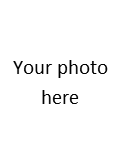
\includegraphics[width=1in,height=1.25in,clip,keepaspectratio]{a1.png}}]{First A. Author} (M'76--SM'81--F'87) and all authors may include 
biographies. Biographies are often not included in conference-related
papers. This author became a Member (M) of IEEE in 1976, a Senior
Member (SM) in 1981, and a Fellow (F) in 1987. The first paragraph may
contain a place and/or date of birth (list place, then date). Next,
the author's educational background is listed. The degrees should be
listed with type of degree in what field, which institution, city,
state, and country, and year the degree was earned. The author's major
field of study should be lower-cased. 

The second paragraph uses the pronoun of the person (he or she) and not the 
author's last name. It lists military and work experience, including summer 
and fellowship jobs. Job titles are capitalized. The current job must have a 
location; previous positions may be listed 
without one. Information concerning previous publications may be included. 
Try not to list more than three books or published articles. The format for 
listing publishers of a book within the biography is: title of book 
(publisher name, year) similar to a reference. Current and previous research 
interests end the paragraph. The third paragraph begins with the author's 
title and last name (e.g., Dr.\ Smith, Prof.\ Jones, Mr.\ Kajor, Ms.\ Hunter). 
List any memberships in professional societies other than the IEEE. Finally, 
list any awards and work for IEEE committees and publications. If a 
photograph is provided, it should be of good quality, and 
professional-looking. Following are two examples of an author's biography.
\end{IEEEbiography}

\begin{IEEEbiography}[{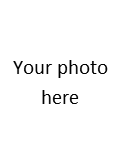
\includegraphics[width=1in,height=1.25in,clip,keepaspectratio]{a2.png}}]{Second B. Author} was born in Greenwich Village, New York, NY, USA in 
1977. He received the B.S. and M.S. degrees in aerospace engineering from 
the University of Virginia, Charlottesville, in 2001 and the Ph.D. degree in 
mechanical engineering from Drexel University, Philadelphia, PA, in 2008.

From 2001 to 2004, he was a Research Assistant with the Princeton Plasma 
Physics Laboratory. Since 2009, he has been an Assistant Professor with the 
Mechanical Engineering Department, Texas A{\&}M University, College Station. 
He is the author of three books, more than 150 articles, and more than 70 
inventions. His research interests include high-pressure and high-density 
nonthermal plasma discharge processes and applications, microscale plasma 
discharges, discharges in liquids, spectroscopic diagnostics, plasma 
propulsion, and innovation plasma applications. He is an Associate Editor of 
the journal \emph{Earth, Moon, Planets}, and holds two patents. 

Dr. Author was a recipient of the International Association of Geomagnetism 
and Aeronomy Young Scientist Award for Excellence in 2008, and the IEEE 
Electromagnetic Compatibility Society Best Symposium Paper Award in 2011. 
\end{IEEEbiography}

\begin{IEEEbiography}[{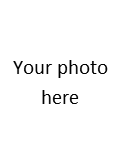
\includegraphics[width=1in,height=1.25in,clip,keepaspectratio]{a3.png}}]{Third C. Author, Jr.} (M'87) received the B.S. degree in mechanical 
engineering from National Chung Cheng University, Chiayi, Taiwan, in 2004 
and the M.S. degree in mechanical engineering from National Tsing Hua 
University, Hsinchu, Taiwan, in 2006. He is currently pursuing the Ph.D. 
degree in mechanical engineering at Texas A{\&}M University, College 
Station, TX, USA.

From 2008 to 2009, he was a Research Assistant with the Institute of 
Physics, Academia Sinica, Tapei, Taiwan. His research interest includes the 
development of surface processing and biological/medical treatment 
techniques using nonthermal atmospheric pressure plasmas, fundamental study 
of plasma sources, and fabrication of micro- or nanostructured surfaces. 

Mr. Author's awards and honors include the Frew Fellowship (Australian 
Academy of Science), the I. I. Rabi Prize (APS), the European Frequency and 
Time Forum Award, the Carl Zeiss Research Award, the William F. Meggers 
Award and the Adolph Lomb Medal (OSA).
\end{IEEEbiography}

\EOD

\end{document}
